\documentclass{beamer}
\usefonttheme[onlymath]{serif}

\usepackage{amsfonts}

% Code Block Setting
\usepackage{listings}
\lstset{language=C,
numberstyle=\footnotesize,
basicstyle=\ttfamily\footnotesize,
numbers=left,
stepnumber=1,
frame=shadowbox,
breaklines=true}

\usetheme{Warsaw}
% \usecolortheme{dove}

% Add frame number and total frame number in footline
\defbeamertemplate*{footline}{shadow theme}{%
    \leavevmode%
    \hbox{\begin{beamercolorbox}[wd=.5\paperwidth,ht=2.5ex,dp=1.125ex,leftskip=.3cm plus1fil,rightskip=.3cm]{author in head/foot}%
            \usebeamerfont{author in head/foot}\hfill\insertshortauthor
        \end{beamercolorbox}%
        \begin{beamercolorbox}[wd=.4\paperwidth,ht=2.5ex,dp=1.125ex,leftskip=.3cm,rightskip=.3cm plus1fil]{title in head/foot}%
            \usebeamerfont{title in head/foot}\insertshorttitle\hfill%
        \end{beamercolorbox}%
        \begin{beamercolorbox}[wd=.1\paperwidth,ht=2.5ex,dp=1.125ex,leftskip=.3cm,rightskip=.3cm plus1fil]{title in head/foot}%
            \hfill\insertframenumber\,/\,\inserttotalframenumber
    \end{beamercolorbox}}%
    \vskip0pt%
}

% Tikz related
\usepackage{tikz}
\usetikzlibrary{fit}
\usetikzlibrary{calc}
\usetikzlibrary{positioning}

% Number the figures
\setbeamertemplate{caption}[numbered]

% Add outline page at begining of each section
\AtBeginSection[]
{
    \begin{frame}<beamer>
        \frametitle{Outline}
        \tableofcontents[currentsection, hideallsubsections]
    \end{frame}
}

%%%%%%%%%%%%%%%%%%%%%%%%%%%%%%%%%%%%%%%%%%%%%

\title{Heterogeneity-aware Distributed Parameter Servers}
\author{
    Jiawei Jiang\inst{1},\\
	Bin Cui\inst{1},\\
    Ce Zhang\inst{2},\\
    Lele Yu\inst{1},\\
}
\institute{
    \inst{1} Peking University
	\inst{2} Department of Computer Science
}
\date{
    \tiny{SIGMOD'17, May 14-19, 2017, Chicago, Illinois, USA}\\
    \tiny{Presented by Ching-Yuan, Tsai}
}

\begin{document}
\begin{frame}
    \titlepage
\end{frame}

\section{Introduction}

\subsection{SIMD}
\begin{frame}
    \frametitle{SIMD}
	\begin{itemize}
		\item Single instruction multiple data
		\item without threads support
	\end{itemize}
\end{frame}


\subsection{VPU}
\begin{frame}
    \frametitle{VPU}
	\begin{itemize}
		\item Vector processing units 
		\item combine itstructions as vector	
	    \begin{figure}
			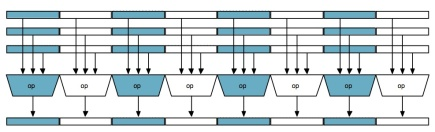
\includegraphics[scale=0.5]{figure/vpu.jpg}
		\end{figure}
	\end{itemize}
\end{frame}


\section{Preliminaries}

\subsection{Destributed SGD}
\begin{frame}
    \frametitle{Destributed SGD}
	\begin{figure}
		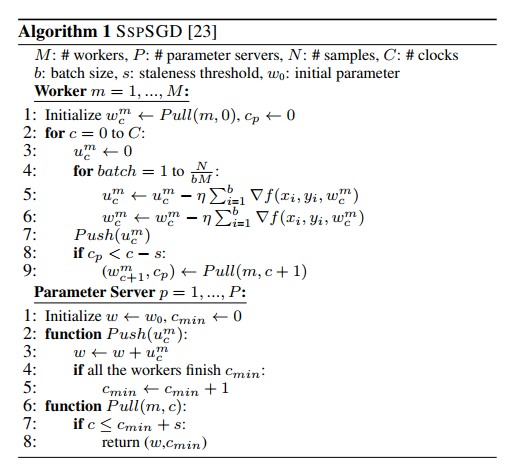
\includegraphics[scale=0.45]{figure/sgd.png}
	\end{figure}
\end{frame}

\subsection{Instroduction of existing systems}
\begin{frame}
    \frametitle{Instroduction of existing systems}
	\begin{itemize}
		\item BSP system: Bulk Synchronous Parallel. 
		\item ASP system: Asynchronous Parallel.
		\item SSP system: Stale Synchronous Parallel. 
	\end{itemize} 
\end{frame}
		
\subsection{Modeling Heterogeneous Clusters}
\begin{frame}
    \frametitle{HL}
	\begin{itemize}
		\item Decomposing the run time of worker into the computation time $t_{c}^{m}$, the transmission time $t_{t}^{m}$.
		\item The heterogeneous level of the cluster is measured by the speed gap between the fastest weorker and the slowest worker.
			\begin{itemize}
				\item $HL = \frac{t_{c}^{s}+t_{t}^{s}}{t_{c}^{f}+t_{t}^{f}}\qquad$
			\end{itemize}
	\end{itemize} 
\end{frame}

\subsection{Experiment on existing systems}
\begin{frame}
    \frametitle{Experiment}
	\begin{itemize}
		\item BSP:Spark, ASP:Petuum, SSP:Bosen. 
		\item They activate the sleep() function in 20\%workers to simulate the heterogeneous environment. 
	\end{itemize}
	\begin{figure}
		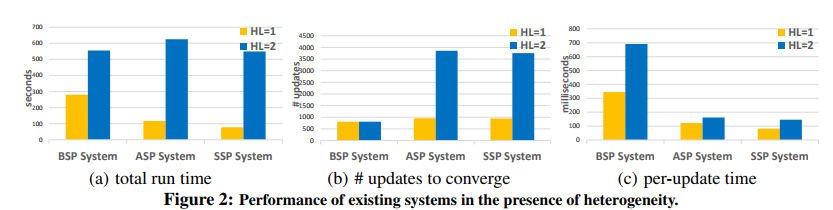
\includegraphics[scale=0.4]{figure/experiment_exist.png}
	\end{figure}
\end{frame}



\section{CONSGD}

\subsection{Algorithm}
\begin{frame}
    \frametitle{Algorithm}
	\begin{itemize}
		\item CONSGD uses a constant global learning rate and multiplies it to each local update. 
		\item $w\gets w+\lambda u_{c}^{m} $, $\lambda \in (0,1)$
	\end{itemize}
\end{frame}

\subsection{Intuition}
\begin{frame}
    \frametitle{Intuition}
	\begin{figure}
		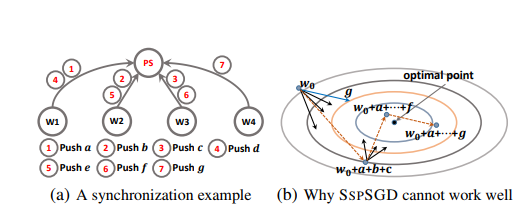
\includegraphics[scale=0.5]{figure/intuition.png}
	\end{figure} 
\end{frame}

\begin{frame}
	\frametitle{Why CONSGD works better?}
	\begin{figure}
		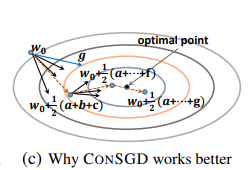
\includegraphics[scale=0.8]{figure/consgdwork.png}
	\end{figure}
\end{frame}



\subsection{Choose $\lambda$}
\begin{frame}
    \frametitle{Choose $\lambda$}
	\begin{itemize}
		\item $w_{c+1}=\frac{1}{M}\sum_{i=1}^{M}(w_{c}+u_{c}^{i})=w_{c}+\frac{1}{M}\sum_{i=1}^{M}u_{c}^{i}$
		\item $\lambda = \frac{1}{M}$ is a good choice. 
	\end{itemize} 
\end{frame}

\subsection{Limitation}
\begin{frame}
    \frametitle{Limitation}
	\begin{figure}
		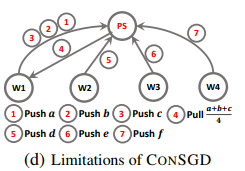
\includegraphics[scale=0.8]{figure/consgdlimit.png}
	\end{figure}
\end{frame}



\section{DYNSGD}

\subsection{Abstract Model of a Parameter Server}
\begin{frame}
    \frametitle{Abstract Model of a Parameter Server}
	\begin{itemize}
		\item Denote PS as a tuple $(S, f_{clock}, f_{server}, \lambda, w_{0})$ ,where S is a stream of updates $\{u_{1}u_{2}...\}.$
		\item $staleness(u_{i})=|\{u_{j}:f_{clock}(j)=f_{clock}(i)\}|.$
		\item $\lambda(i)=\frac{1}{staleness(i)}$
		\item $w(PS, i)=w_{0}+\sum_{j}\lambda(j)u_{j},   \forall f_{clock}(j)<i.$
		\item $u(PS, i)= \sum_{j}\lambda(j)u_{j},   \forall f_{clock}(j)=i.$
			\begin{itemize}
				\item $w(PS,i+1) = w(PS, i) + u(PS, i)$
			\end{itemize}
	\end{itemize}
\end{frame}
\begin{frame}
	\frametitle{Intuition}
	\begin{figure}
		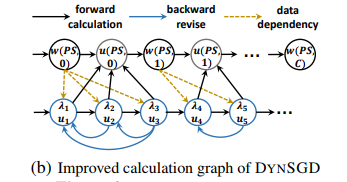
\includegraphics[scale=0.8]{figure/intuitiondynsgd.png}
	\end{figure}
\end{frame}
\begin{frame}
	\begin{figure}
		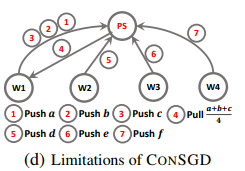
\includegraphics[scale=0.8]{figure/consgdlimit.png}
	\end{figure}
\end{frame}




\subsection{Implementation of DYNSGD}
\begin{frame}
    \frametitle{Fast staleness computing}
	\begin{itemize}
		\item $V(m)$: the version of the local update from worker m.
		\item $S(v)$: the staleness of the local update stamped with version v.
		\item $staleness(u_{c}^{m}) = S(V(m))$
		\item $\Delta u = \frac{1}{d}u_{c}^{m}+\frac{d-1}{d}u(PS,v)-u(PS,v)=\frac{1}{d}(u_{c}^{m}-u(PC,v))$
	\end{itemize} 
\end{frame}




\subsection{Algorithm}
\begin{frame}
    \frametitle{Algorithm}
	\begin{figure}
		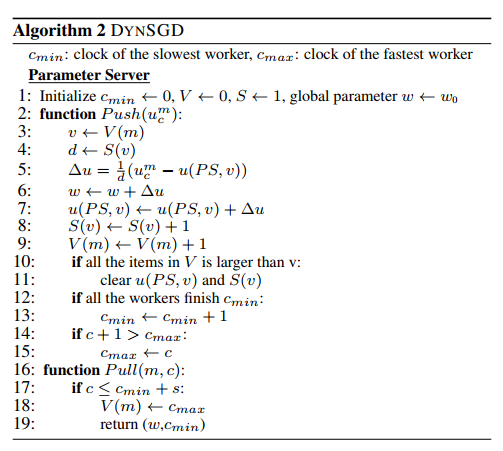
\includegraphics[scale=0.5]{figure/dynsgd.png}
	\end{figure} 
\end{frame}

\subsection{Partition Synchronization}
\begin{frame}
    \frametitle{Partition Synchronization}
	\begin{figure}
		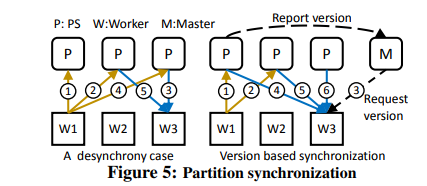
\includegraphics[scale=0.8]{figure/partitionsyn.png}
	\end{figure} 
\end{frame}




\section{Experiment and Conclusion}

\subsection{Experiment}
\begin{frame}
    \frametitle{Experiment}
	\begin{figure}
		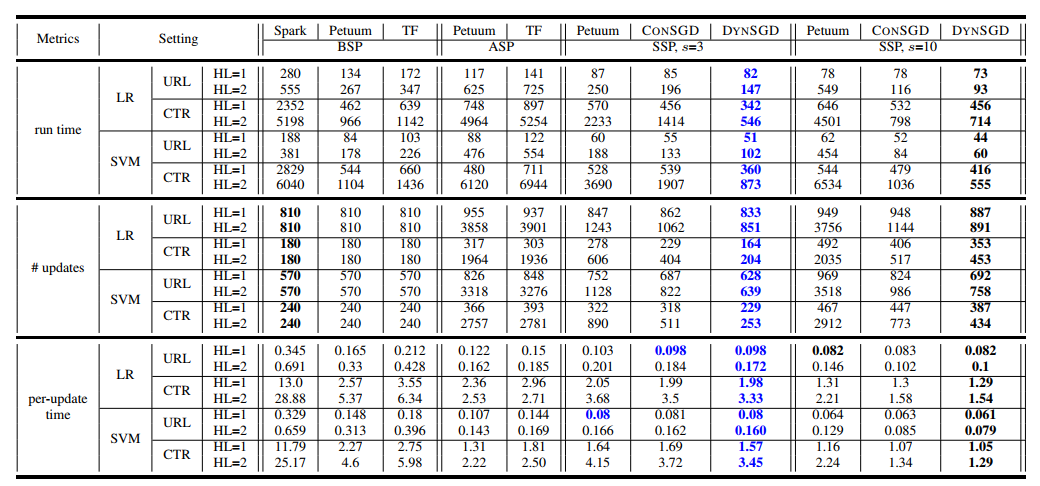
\includegraphics[scale=0.3]{figure/experiment.png}
	\end{figure}
\end{frame}

\subsection{Conclusion}
\begin{frame}
	\frametitle{Conclusion}
	\begin{itemize}
		\item They proposed two heterogeneity-aware distributed SGD algorithms under SSP protocol.
	\end{itemize} 
\end{frame}

\subsection{Future Work}
\begin{frame}
	\frametitle{Future Work}
	\begin{itemize}
		\item Normalizeing updates. 
	\end{itemize}
\end{frame}




\end{document}
